% ============================================================
\chapter{Bifurcations}
\label{ch:bifurcations}
% ============================================================

Imaginez un syst\`eme physique qui d\'epend d'un param\`etre~: la charge sur un pont, la temp\'erature d'un fluide, le taux de natalit\'e d'une population. \`A mesure que le param\`etre varie, le comportement du syst\`eme change progressivement --- jusqu'\`a un seuil critique o\`u tout bascule~: un \'equilibre stable dispara\^it, un cycle limite appara\^it, le nombre de solutions change brusquement. Ce changement qualitatif soudain est une \emph{bifurcation}, et sa classification --- n\oe ud-selle, transcritique, fourche, Hopf --- constitue l'un des chapitres les plus beaux de la th\'eorie des syst\`emes dynamiques, h\'erit\'e des travaux de Poincar\'e et syst\'ematis\'e par Ren\'e Thom dans sa \emph{th\'eorie des catastrophes} (1972).

\section{Introduction}

Une \textbf{bifurcation} se produit lorsque la structure qualitative du
portrait de phase d'un syst\`eme dynamique change sous l'effet de la variation
d'un param\`etre. Ce chapitre \'etudie les bifurcations locales les plus
fondamentales : n\oe ud-col, transcritique, fourche et Hopf.

\section{Cadre g\'en\'eral}

\begin{definition}[Bifurcation]
Consid\'erons le syst\`eme param\'etrique $\dot{x} = f(x, \mu)$, o\`u
$x \in \R^n$ et $\mu \in \R^p$ est un vecteur de param\`etres. Une valeur
$\mu_0$ est une \textbf{valeur de bifurcation} si le portrait de phase de
$f(\cdot, \mu)$ n'est pas topologiquement \'equivalent pour $\mu$ pr\`es de
$\mu_0$ de part et d'autre.
\end{definition}

\begin{definition}[Bifurcation locale]
Une bifurcation est \textbf{locale} si elle est associ\'ee au changement de
stabilit\'e d'un point d'\'equilibre, c'est-\`a-dire au passage d'une valeur
propre de la jacobienne \`a travers l'axe imaginaire.
\end{definition}

\begin{definition}[Codimension]
La \textbf{codimension} d'une bifurcation est le nombre minimal de
param\`etres ind\'ependants n\'ecessaires pour l'observer de mani\`ere
g\'en\'erique.
\end{definition}

\section{Bifurcation n\oe ud-col (saddle-node)}

\begin{definition}[Bifurcation n\oe ud-col]
La \textbf{bifurcation n\oe ud-col} (ou \textbf{pli}) est la cr\'eation ou
l'annihilation de deux points d'\'equilibre lorsqu'un param\`etre traverse
une valeur critique.
\end{definition}

\begin{theoreme}[Forme normale du n\oe ud-col]
\label{thm:saddle-node}
La forme normale de la bifurcation n\oe ud-col en dimension 1 est
\[
    \dot{x} = \mu + x^2.
\]
\begin{itemize}
    \item Pour $\mu < 0$ : deux \'equilibres $x^* = \pm\sqrt{-\mu}$
    (un stable, un instable).
    \item Pour $\mu = 0$ : un \'equilibre semi-stable $x^* = 0$.
    \item Pour $\mu > 0$ : aucun \'equilibre.
\end{itemize}
\end{theoreme}

\begin{theoreme}[Conditions du n\oe ud-col]
Soit $\dot{x} = f(x, \mu)$ avec $f(x_0, \mu_0) = 0$. La bifurcation
n\oe ud-col se produit en $(x_0, \mu_0)$ si :
\begin{enumerate}
    \item $\frac{\partial f}{\partial x}(x_0, \mu_0) = 0$ (valeur propre nulle) ;
    \item $\frac{\partial f}{\partial \mu}(x_0, \mu_0) \neq 0$ (transversalit\'e) ;
    \item $\frac{\partial^2 f}{\partial x^2}(x_0, \mu_0) \neq 0$ (non-d\'eg\'en\'erescence).
\end{enumerate}
\end{theoreme}

% Diagramme de bifurcation
\begin{center}
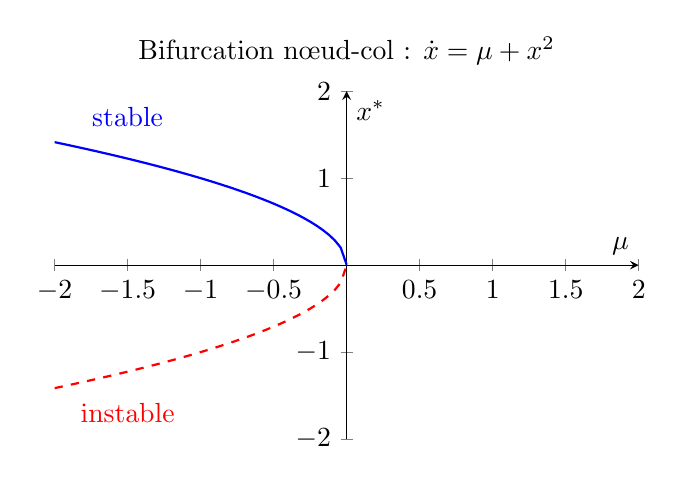
\begin{tikzpicture}
    \begin{axis}[
        width=9cm, height=6cm,
        xlabel={$\mu$}, ylabel={$x^*$},
        xmin=-2, xmax=2, ymin=-2, ymax=2,
        axis lines=middle,
        title={Bifurcation n\oe ud-col : $\dot{x} = \mu + x^2$}
    ]
    \addplot[blue, thick, domain=-2:0, samples=50] {sqrt(-x)};
    \addplot[red, thick, dashed, domain=-2:0, samples=50] {-sqrt(-x)};
    \node[blue] at (axis cs:-1.5,1.7) {stable};
    \node[red] at (axis cs:-1.5,-1.7) {instable};
    \end{axis}
\end{tikzpicture}
\end{center}

\section{Bifurcation transcritique}

\begin{definition}[Bifurcation transcritique]
Dans une \textbf{bifurcation transcritique}, deux \'equilibres \'echangent
leur stabilit\'e au point de bifurcation, sans cr\'eation ni disparition.
\end{definition}

\begin{theoreme}[Forme normale transcritique]
La forme normale est $\dot{x} = \mu x - x^2$.
\begin{itemize}
    \item Pour $\mu < 0$ : $x^* = 0$ stable, $x^* = \mu$ instable.
    \item Pour $\mu > 0$ : $x^* = 0$ instable, $x^* = \mu$ stable.
\end{itemize}
Les deux branches d'\'equilibre se croisent en $\mu = 0$ et \'echangent
leur stabilit\'e.
\end{theoreme}

\begin{exemple}[Mod\`ele logistique avec r\'ecolte constante]
Le mod\`ele $\dot{N} = rN(1 - N/K) - H$ pr\'esente une bifurcation
n\oe ud-col lorsque $H$ augmente : au-del\`a d'un seuil critique, la
population s'effondre.
\end{exemple}

\section{Bifurcation fourche (pitchfork)}

\begin{definition}[Bifurcation fourche]
La \textbf{bifurcation fourche} se produit dans les syst\`emes poss\'edant
une sym\'etrie $x \mapsto -x$. Un \'equilibre perd sa stabilit\'e et donne
naissance \`a deux nouveaux \'equilibres.
\end{definition}

\begin{theoreme}[Bifurcation fourche surcritique]
La forme normale est $\dot{x} = \mu x - x^3$.
\begin{itemize}
    \item Pour $\mu \leq 0$ : seul $x^* = 0$ existe, stable.
    \item Pour $\mu > 0$ : $x^* = 0$ instable, deux nouveaux \'equilibres
    stables $x^* = \pm\sqrt{\mu}$.
\end{itemize}
\end{theoreme}

\begin{theoreme}[Bifurcation fourche sous-critique]
La forme normale est $\dot{x} = \mu x + x^3$.
\begin{itemize}
    \item Pour $\mu < 0$ : $x^* = 0$ stable, deux \'equilibres instables
    $x^* = \pm\sqrt{-\mu}$.
    \item Pour $\mu \geq 0$ : seul $x^* = 0$ existe, instable.
\end{itemize}
La bifurcation sous-critique est \textbf{dangereuse} car l'\'equilibre perd
brusquement sa stabilit\'e sans alternative stable locale.
\end{theoreme}

\begin{center}
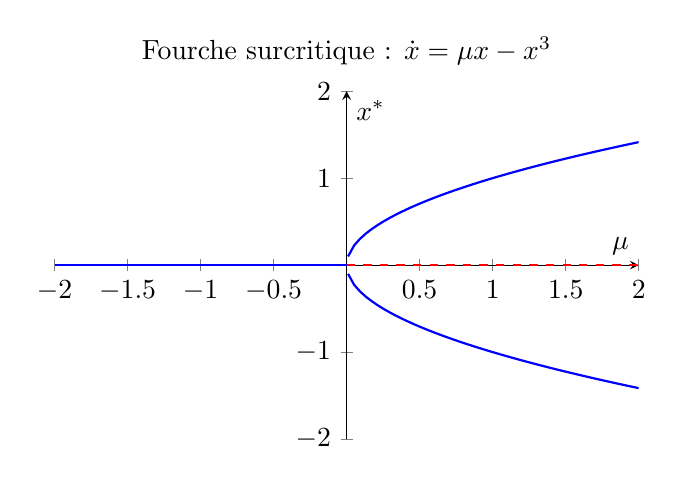
\begin{tikzpicture}
    \begin{axis}[
        width=9cm, height=6cm,
        xlabel={$\mu$}, ylabel={$x^*$},
        xmin=-2, xmax=2, ymin=-2, ymax=2,
        axis lines=middle,
        title={Fourche surcritique : $\dot{x} = \mu x - x^3$}
    ]
    % Branche triviale stable (mu < 0)
    \addplot[blue, thick, domain=-2:0, samples=20] {0};
    % Branche triviale instable (mu > 0)
    \addplot[red, thick, dashed, domain=0:2, samples=20] {0};
    % Branches non triviales
    \addplot[blue, thick, domain=0.01:2, samples=50] {sqrt(x)};
    \addplot[blue, thick, domain=0.01:2, samples=50] {-sqrt(x)};
    \end{axis}
\end{tikzpicture}
\end{center}

\begin{exemple}[Flambage d'Euler]
La d\'eflexion d'une poutre sous charge axiale $P$ est gouvern\'ee par
\[
    EI\frac{d^2\theta}{ds^2} + P\sin\theta = 0.
\]
Lin\'earis\'e, cela donne une bifurcation fourche surcritique \`a
$P_c = \pi^2 EI / L^2$ (charge critique d'Euler).
\end{exemple}

\section{Bifurcation de Hopf}

\begin{definition}[Bifurcation de Hopf]
La \textbf{bifurcation de Hopf} se produit lorsqu'une paire de valeurs
propres complexes conjugu\'ees traverse l'axe imaginaire. Elle donne naissance
\`a un cycle limite (ou le d\'etruit).
\end{definition}

\begin{theoreme}[Hopf]
\label{thm:hopf}
Soit $\dot{x} = f(x, \mu)$ avec $f(0, \mu) = 0$ pour tout $\mu$ et
$A(\mu) = D_x f(0, \mu)$ ayant des valeurs propres
$\lambda(\mu) = \alpha(\mu) \pm i\beta(\mu)$. Supposons :
\begin{enumerate}
    \item $\alpha(0) = 0$, $\beta(0) = \omega_0 \neq 0$
    (valeurs propres sur l'axe imaginaire) ;
    \item $\alpha'(0) \neq 0$ (condition de transversalit\'e : les valeurs
    propres traversent l'axe imaginaire avec une vitesse non nulle).
\end{enumerate}
Alors :
\begin{itemize}
    \item \textbf{Hopf surcritique} (premier coefficient de Lyapunov $\ell_1 < 0$) :
    un cycle limite \textbf{stable} na\^it pour $\mu > 0$ (l'\'equilibre
    devient instable) ;
    \item \textbf{Hopf sous-critique} ($\ell_1 > 0$) :
    un cycle limite \textbf{instable} existe pour $\mu < 0$ (l'\'equilibre
    est encore stable), et dispara\^it \`a $\mu = 0$.
\end{itemize}
\end{theoreme}

\begin{formules}[title=\textbf{Premier coefficient de Lyapunov}]
Pour le syst\`eme $\dot{z} = (\alpha + i\omega)z + c_1 z\abs{z}^2 + \cdots$
en coordonn\'ees complexes, le premier coefficient de Lyapunov est
$\ell_1 = \text{Re}(c_1)$. Si $\ell_1 < 0$ la bifurcation est surcritique.
\end{formules}

\begin{exemple}[Oscillateur de Stuart-Landau]
Le mod\`ele $\dot{z} = (\mu + i\omega)z - z\abs{z}^2$ en coordonn\'ees
polaires $(r, \theta)$ donne
\[
    \dot{r} = \mu r - r^3, \qquad \dot{\theta} = \omega.
\]
Pour $\mu > 0$, un cycle limite stable de rayon $r = \sqrt{\mu}$ existe.
C'est la bifurcation de Hopf surcritique par excellence.
\end{exemple}

\begin{codeblock}[title=\textbf{Diagramme de bifurcation et Hopf}]
\begin{minted}{python}
import numpy as np
from scipy.integrate import solve_ivp
import matplotlib.pyplot as plt

def hopf_system(t, state, mu):
    x, y = state
    r2 = x**2 + y**2
    return [mu*x - y - x*r2, x + mu*y - y*r2]

fig, axes = plt.subplots(1, 3, figsize=(15, 5))
mus = [-0.5, 0.0, 0.5]
for ax, mu in zip(axes, mus):
    for r0 in [0.1, 0.3, 0.8, 1.5, 2.0]:
        for th in [0, np.pi/2, np.pi, 3*np.pi/2]:
            x0 = [r0*np.cos(th), r0*np.sin(th)]
            sol = solve_ivp(hopf_system, [0, 30], x0,
                            args=(mu,), max_step=0.05)
            ax.plot(sol.y[0], sol.y[1], 'b-', lw=0.3)
    ax.set_title(f"$\\mu = {mu}$")
    ax.set_xlim(-2, 2); ax.set_ylim(-2, 2)
    ax.set_aspect('equal'); ax.grid(True, alpha=0.3)
plt.suptitle("Bifurcation de Hopf surcritique", fontsize=14)
plt.tight_layout()
plt.savefig("hopf_bifurcation.pdf")
plt.show()
\end{minted}
\end{codeblock}

\section{Diagrammes de bifurcation}

\begin{definition}[Diagramme de bifurcation]
Un \textbf{diagramme de bifurcation} repr\'esente les \'equilibres (ou
amplitudes des cycles) en fonction du param\`etre $\mu$. Les branches
stables sont trac\'ees en trait plein, les branches instables en pointill\'e.
\end{definition}

\begin{remarque}
Pour les bifurcations de Hopf, on repr\'esente g\'en\'eralement le rayon du
cycle limite (ou le maximum/minimum d'une composante) en fonction de $\mu$.
\end{remarque}

\section{Bifurcations globales}

\begin{definition}[Bifurcation homocline]
Une \textbf{bifurcation homocline} se produit lorsqu'une orbite homocline
(connexion d'un col \`a lui-m\^eme) appara\^it ou dispara\^it. Elle peut
engendrer un cycle limite de grande p\'eriode.
\end{definition}

\begin{definition}[Bifurcation SNIC]
La bifurcation \textbf{SNIC} (Saddle-Node on an Invariant Circle) se produit
lorsqu'un n\oe ud-col appara\^it sur un cycle limite, le d\'etruisant.
La p\'eriode du cycle tend vers l'infini \`a la bifurcation.
\end{definition}

\begin{theoreme}[Scaling de la p\'eriode]
\begin{itemize}
    \item Bifurcation SNIC : $T \sim \frac{1}{\sqrt{\mu - \mu_c}}$ ;
    \item Bifurcation homocline : $T \sim -\frac{1}{\lambda_s}\ln\abs{\mu - \mu_c}$,
    o\`u $\lambda_s$ est la valeur propre stable du col.
\end{itemize}
\end{theoreme}

\section{Bifurcations en dimension sup\'erieure}

\begin{remarque}
En dimension $n > 2$, les m\^emes bifurcations locales se produisent par
r\'eduction \`a la vari\'et\'e centrale. Les conditions sont identiques mais
s'appliquent au syst\`eme r\'eduit. Des bifurcations sp\'ecifiques
apparaissent aussi :
\begin{itemize}
    \item \textbf{Bogdanov-Takens} (codimension 2) : valeur propre double
    nulle ;
    \item \textbf{Hopf-Hopf} (codimension 2) : deux paires de valeurs
    propres purement imaginaires ;
    \item \textbf{Cusp} (codimension 2) : d\'eg\'en\'erescence du
    n\oe ud-col.
\end{itemize}
\end{remarque}

\section{Applications physiques}

\begin{exemple}[Laser]
Le laser \`a semi-conducteur est mod\'elis\'e par les \'equations de taux :
\[
    \dot{n} = J - n - (1 + 2n)P, \qquad \dot{P} = \gamma\left[(1 + 2n)P - P + \beta n\right].
\]
La transition du laser (sous-seuil vers \'emission laser) est une bifurcation
transcritique. Pour certains mod\`eles avec r\'etroaction optique, une
bifurcation de Hopf engendre des oscillations.
\end{exemple}

\section{Exercices}

\begin{exercice}[N\oe ud-col en dimension 2]
\'Etudier les bifurcations du syst\`eme
$\dot{x} = \mu - x^2$, $\dot{y} = -y$. Tracer le diagramme de bifurcation.
\end{exercice}

\begin{exercice}[Fourche avec imperfection]
Consid\'erer $\dot{x} = h + \mu x - x^3$ avec $h$ petit. Montrer que
l'imperfection $h$ brise la sym\'etrie de la bifurcation fourche et
tracer le diagramme dans le plan $(\mu, x^*)$ pour $h > 0$.
\end{exercice}

\begin{exercice}[Hopf dans un syst\`eme chimique]
Pour le syst\`eme de Brusselator $\dot{x} = 1 - (b+1)x + ax^2y$,
$\dot{y} = bx - ax^2y$, trouver la valeur de bifurcation de Hopf
en fonction de $a$ et $b$.
\end{exercice}

\begin{exercice}[Diagramme complet]
Pour $\dot{x} = \mu x + x^3 - x^5$, tracer le diagramme de bifurcation
complet, identifier les bifurcations n\oe ud-col et fourche, et
d\'eterminer la pr\'esence d'hyst\'er\'esis.
\end{exercice}

\begin{exercice}[Bifurcation de Hopf --- calcul]
Calculer le premier coefficient de Lyapunov pour le syst\`eme
$\dot{x} = \mu x - y - x(x^2 + y^2)$,
$\dot{y} = x + \mu y - y(x^2 + y^2)$
et d\'eterminer si la bifurcation est surcritique ou sous-critique.
\end{exercice}

\begin{exercice}[Bifurcation homocline]
Consid\'erer le syst\`eme $\dot{x} = y$, $\dot{y} = x - x^2 + \mu y$.
Montrer qu'une orbite homocline existe pour une valeur particuli\`ere de $\mu$
et discuter la cr\'eation/destruction d'un cycle limite.
\end{exercice}
